%\documentclass[a4paper,12pt,twoside]{report}
\documentclass[a4paper,12pt]{report}

\usepackage{url}
\usepackage{amsmath}
\usepackage{lipsum}
\usepackage{listings}
\usepackage{color}
\usepackage{graphicx}
\usepackage[font=footnotesize, margin=15pt]{caption}

\definecolor{mygreen}{rgb}{0,0.6,0}
\definecolor{mygray}{rgb}{0.6,0.6,0.6}
\definecolor{mymauve}{rgb}{0.58,0,0.82}

\lstset{
  captionpos=b,
  numbers=left,
  frame=tb,
  showstringspaces=false,
  numbersep=15pt,
  xleftmargin=30pt,
  aboveskip=15pt,
  belowskip=15pt,
  keywordstyle=\color{blue},
  stringstyle=\color{mymauve},
  numberstyle=\color{mygray},
  rulecolor=\color{mygray}
}

\title{Resolution of two dimensional collisions}
\author{Philip Burridge\\
        Dan Camarda\\
        Alexander Cederblad\\
        Rasmus Haapaoja\\
        Fredrik Johnson}
\date{\today}


%-- Document
\begin{document}


%-- Title
\maketitle


%-- Abstract
\begin{abstract}
This report will cover the thought process of creating a physics simulation of collision impulses for basic geometries. It will also cover most a couple of numerical methods for integration which is essential for these kinds of simulations.
\end{abstract}


%-- Table of Contents
\tableofcontents
\addtocontents{toc}{\protect\thispagestyle{empty}}
%\listoffigures
%\listoftables
%\lstlistoflistings


%-- Introduction
\chapter{Introduction}
\setcounter{page}{1}

We have chosen a general system involving collision impulse between rigid bodies in two and three dimensions. The implementation of the problem of resolving collisions includes calculating collisions between these bodies. Because of this and the fact that the focus of this project is the physical system and the numerical methods of simulation, the simplest geometries were chosen to narrow the focus. What are the simplest geometries for collision detection, you ask? Circles and spheres are the answer to your question. Since they can only collide at \emph{one} point with other convex geometries, they are the best choice to keep the focus on the simulation. Figure ~\ref{fig:snapshot} show a snapshot of this kind of simulation with circles.

\begin{figure}[!ht]
    \centering
    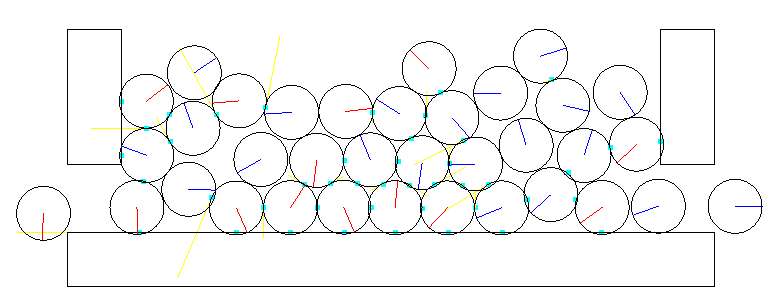
\includegraphics[width=0.8\textwidth]{figures/snapshot.png}
    \caption{A snapshop of a simulation of circles interacting with each other. The line from the origin indicates the angle.}
    \label{fig:snapshot}
\end{figure}


%-- Method
\chapter{Method}

% Collision detection
\section{Collision detection}

To be able to resolve a collision, an actual collision must be registered. As mentioned in the previous chapter, the focus is not put on collision detection. There is some information that we need to know about a collision to be able to resolve the collision impulse in a later step. We need to know the \emph{penetration} of the collision, the \emph{normal} of the collision and the \emph{collision point}. Figure ~\ref{fig:snapshot} displays a collision between two circles including this information.

\begin{figure}[!ht]
    \centering
    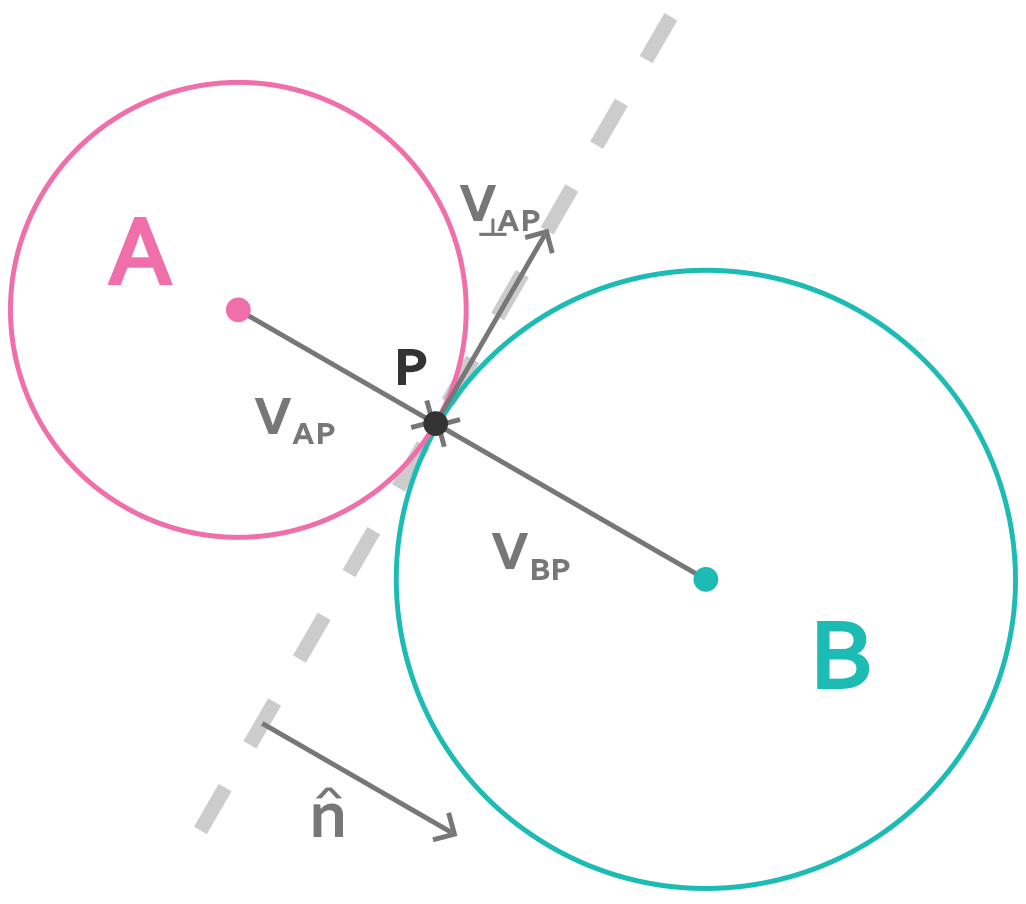
\includegraphics[width=0.6\textwidth]{figures/collision.png}
    \caption{A collision including the normal of the collision and other quantities related to the collision. The collision normal is chosen from A to B by convention.}
    \label{fig:collision}
\end{figure}

% Resolving an impulse
\section{Resolving an impulse}

To explain how to resolve an impulse\cite{gdm}, let us first think about two objects colliding with each other, both with their own seperate velocities. Assume that we know the normal of the collision. During a collision, an instant force (i.e. an \emph{impulse}), will act on both objects, knocking them apart from each other. This change in the object's relative velocity, as explained in \ref{eq:1}, tells us that the relative velocity will be inverted proportional with the \emph{coefficient of restitution} (\emph{e}, which will be covered later on).

\begin{equation}
\mathbf v'_{AB}\cdot \mathbf n=-e\mathbf v_{AB}\cdot \mathbf n
\label{eq:1}
\end{equation}

The above equation is used, among other physical properties, to solve for a coefficient \ref{eq:2} of the impulse that will later be applied to the objects as a way of changing their velocity and angular velocity.

\begin{equation}
j = \dfrac{ -(1+e) \mathbf v_{AB} \cdot \mathbf n }{
    \mathbf n \cdot \mathbf n ( \dfrac{1}{M_{A}} + \dfrac{1}{M_{A}} )
    + \dfrac{ (\mathbf r_{AP\perp} \cdot \mathbf n)^2}{I_{A} }
    + \dfrac{ (\mathbf r_{BP\perp} \cdot \mathbf n)^2}{I_{B} } }
\label{eq:2}
\end{equation}

Now that the impulse coefficient is known, one might think, "how is a scalar going to help us resolve a collision impulse?". The question is legitimate and it will be explained in the following equations (\ref{eq:3} and \ref{eq:4}). The scalar is multiplied with the normalized \emph{collision vector} in both equations.

\begin{equation}
\mathbf v'_{A}=\mathbf v_{A}+\dfrac{j}{M_{A}}\mathbf n
\label{eq:3}
\end{equation}
\begin{equation}
\omega'_{A}=\omega_{A}+\dfrac{\mathbf r_{AP\perp}\cdot j\mathbf n}{I_{A}}
\label{eq:4}
\end{equation}

This is the basic simulation; when a collision occurs, solve for the properties of the collision and then apply the impulse to the objects velocity and angular velocity.

% Resolvning an impulse
\section{Numerical integration}

\subsection{Euler method}

Since computers live in a world of zeroes and ones, we need a to integrate numerically, the most basic and widely used approach is the \emph{Euler method}\cite{gdm}. For this type of simulation, the \emph{Euler method} is suitable for the majority of applications; however, another method will also be covered. The \emph{Euler method} \ref{eq:5} works by adding the current state with its derivative multiplied by the step in time.

\begin{equation}
y_{n+1}=y_{n}+hf(t_n, y_n)
\label{eq:5}
\end{equation}

For example \ref{eq:6} if we are going to integrate a velocity for the next time step, take the current velocity and add it to the acceleration multiplied with the time step.

\begin{equation}
v(t+1)=v(t)+ha(t)
\label{eq:6}
\end{equation}

Since this method is one of the more simplistic numerical methods, it is important to keep in mind that an error will compound with each iteration. Many times the Euler method is not good enough, the compound error increase as long as the simulation is running, as explained by \cite{gog}.

\subsection{Runge Kutta method}

This section is not yet finished.

% OpenGL Implementation
\section{OpenGL implementation}

The chosen method to run the simulation is \emph{OpenGL} which is a computer graphics API for most graphics cards. Our implementation was written in \emph{C++}. Listing \ref{lst:1} shows pseudo code for the implementation.

\begin{lstlisting}[caption={Pseudo code for the simulation loop.}, label=lst:1]
while simulation running:
    find collisions;
    apply gravitational force;
    resolve collision impulse;
    integrate resolved velocities;
    update position;
    draw objects at new position;
\end{lstlisting}

\subsection{Running the simulation}
Navigate to the folder with your current operating system and click the executable file named $simulation$ to run the simulation. The software is not tested on any Linux distribution.

\subsubsection{Requirements}
\begin{itemize}
    \item Graphics card from this century
\end{itemize}


%-- Discussion
\chapter{Discussion}

This section is not finished.


%-- Bibliography
\bibliographystyle{vancouver}
\bibliography{report}


%-- End of Document
\end{document}
